\normaltrue
\correctionfalse

%\UPSTIidClasse{11} % 11 sup, 12 spé
%\newcommand{\UPSTIidClasse}{12}

\exer{Mouvement RT  $\star$ \label{CIN:02:B2:13:06}}
\setcounter{question}{0}\marginnote{\xpComp{CIN}{02}%\xpComp{CIN}{02}%\UPSTIcompetence[2]{C2-05}
%\UPSTIcompetence[2]{B2-13}
}
\index{Compétence C2-05}
\index{Compétence B2-13}\index{Compétence CIN-02}
\index{Mécanisme à 1 translation et 1 rotation}
\ifcorrection
\else
\marginnote{\textbf{Pas de corrigé pour cet exercice.}}
\fi

\ifprof
\else
Soit le mécanisme suivant. On a $\vect{AB}=\lambda(t)\vect{i_0}$ et $\vect{BC}=R\vect{i_2}$ avec $R=\SI{30}{mm}$. 
\begin{marginfigure}
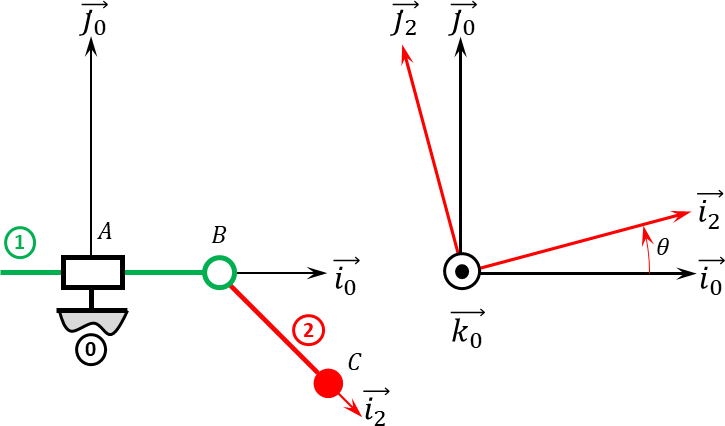
\includegraphics[width=.8\linewidth]{06_TR_01}
\end{marginfigure}
\fi

\question{Donner l'ensemble des positions accessibles par le point $B$.}
\ifprof
\else
\fi

\question{Donner l'équation horaire (trajectoire en fonction du temps) du point $B$ dans le mouvement de \textbf{2} par rapport à \textbf{0}.}
\ifprof
\else
\fi

On souhaite que le point $B$ réalise un segment entre les points $[-25,25]$ et $[25,25]$. 

\question{Donner les expressions de $\theta(t)$ et $\lambda(t)$ permettant la réalisation de cette trajectoire à la vitesse $v=\SI{0,01}{m.s^{-1}}$.}
\ifprof
\else
\fi

\question{En utilisant Python, tracer $\theta(t)$, $\lambda(t)$ et la trajectoire générée.}
\ifprof
\else
\fi


\ifprof
\else
\marginnote{Corrigé  voir \ref{CIN:02:B2:13:06}.}
\fi